% Fichier : sections/02_architecture.tex
\section{Architecture Système et Conception}

\subsection{Vue d'ensemble de l'architecture}

L'architecture de Running App repose sur une approche moderne en trois couches qui sépare clairement les responsabilités et facilite la maintenance ainsi que l'évolutivité du système. Cette conception architecturale s'inspire des meilleures pratiques de développement d'applications mobiles et web, en privilégiant la modularité, la scalabilité et la sécurité.

La première couche correspond à l'interface utilisateur développée en React Native, qui assure une expérience native sur les plateformes iOS et Android tout en permettant un développement unifié. Cette couche gère l'affichage des données, les interactions utilisateur et la communication avec les services du téléphone comme le GPS et les capteurs de mouvement.

La deuxième couche constitue l'API REST développée avec Flask, qui centralise toute la logique métier de l'application. Cette API expose des endpoints sécurisés pour la gestion des utilisateurs, l'enregistrement des courses, la génération de statistiques et la proposition de nouveaux entraînements. Elle implémente également tous les mécanismes d'authentification et d'autorisation nécessaires à la sécurité du système.

La troisième couche représente la base de données MySQL qui stocke de manière persistante toutes les informations de l'application. Cette base de données est conçue pour optimiser les performances lors des requêtes fréquentes tout en maintenant l'intégrité des données grâce à un système de contraintes et de relations bien définies.

\begin{infobox}[Principe architectural]
L'architecture en couches permet une séparation claire des préoccupations: l'interface se concentre sur l'expérience utilisateur, l'API gère la logique métier et la sécurité, tandis que la base de données optimise le stockage et la récupération des informations.
\end{infobox}

\subsection{Architecture client-serveur détaillée}

Notre système implémente une architecture client-serveur moderne qui tire parti des avantages de chaque plateforme tout en maintenant une cohérence fonctionnelle entre les environnements.

Du côté client, l'application React Native utilise une architecture basée sur des composants réutilisables qui encapsulent leur logique et leur présentation. Cette approche facilite la maintenance du code et permet une évolution incrémentale de l'interface utilisateur. Les composants communiquent entre eux via un système de propriétés et d'événements, tandis qu'un gestionnaire d'état global maintient la cohérence des données à travers l'application.

La gestion des données côté client s'appuie sur un système de cache intelligent qui minimise les appels réseau et améliore les performances perçues par l'utilisateur. Les données de course sont stockées localement pendant l'enregistrement pour éviter toute perte en cas de connectivité intermittente, puis synchronisées avec le serveur dès que la connexion est rétablie.

Du côté serveur, l'API Flask adopte une architecture modulaire organisée en blueprints qui regroupent les fonctionnalités par domaine métier. Cette organisation facilite la collaboration entre développeurs et permet une montée en charge progressive du système. Chaque blueprint encapsule ses routes, ses modèles de données et sa logique métier spécifique.

Le serveur implémente également un système de middleware qui traite de manière transversale des préoccupations comme l'authentification, la journalisation des requêtes, la gestion des erreurs et l'ajout des en-têtes de sécurité. Cette approche garantit une application cohérente de ces mécanismes sur l'ensemble de l'API.

\subsection{Diagramme d'architecture système}

\begin{figure}[h]
\centering
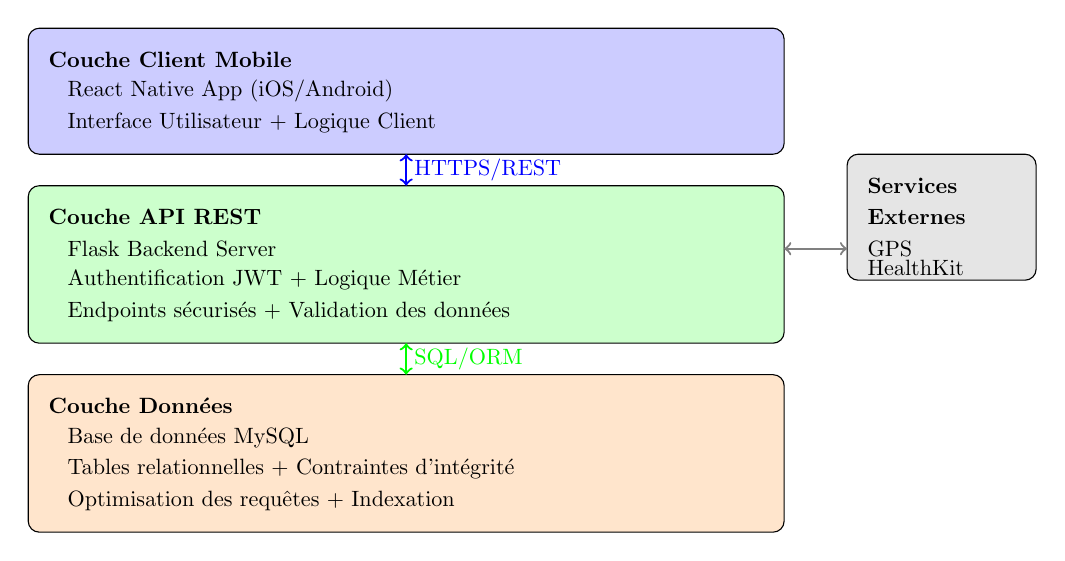
\begin{tikzpicture}[scale=0.8, every node/.style={scale=0.8}]

% Couche Client Mobile
\draw[fill=blue!20, rounded corners] (0,8) rectangle (12,10);
\node[anchor=west] at (0.2,9.5) {\textbf{Couche Client Mobile}};
\node[anchor=west] at (0.5,9) {React Native App (iOS/Android)};
\node[anchor=west] at (0.5,8.5) {Interface Utilisateur + Logique Client};

% Couche API/Middleware
\draw[fill=green!20, rounded corners] (0,5) rectangle (12,7.5);
\node[anchor=west] at (0.2,7) {\textbf{Couche API REST}};
\node[anchor=west] at (0.5,6.5) {Flask Backend Server};
\node[anchor=west] at (0.5,6) {Authentification JWT + Logique Métier};
\node[anchor=west] at (0.5,5.5) {Endpoints sécurisés + Validation des données};

% Couche Base de Données
\draw[fill=orange!20, rounded corners] (0,2) rectangle (12,4.5);
\node[anchor=west] at (0.2,4) {\textbf{Couche Données}};
\node[anchor=west] at (0.5,3.5) {Base de données MySQL};
\node[anchor=west] at (0.5,3) {Tables relationnelles + Contraintes d'intégrité};
\node[anchor=west] at (0.5,2.5) {Optimisation des requêtes + Indexation};

% Flèches de communication
\draw[<->, thick, blue] (6,7.5) -- (6,8) node[midway,right] {HTTPS/REST};
\draw[<->, thick, green] (6,4.5) -- (6,5) node[midway,right] {SQL/ORM};

% Services externes
\draw[fill=gray!20, rounded corners] (13,6) rectangle (16,8);
\node[anchor=west] at (13.2,7.5) {\textbf{Services}};
\node[anchor=west] at (13.2,7) {\textbf{Externes}};
\node[anchor=west] at (13.2,6.5) {GPS};
\node[anchor=west] at (13.2,6.2) {HealthKit};

\draw[<->, thick, gray] (12,6.5) -- (13,6.5);

\end{tikzpicture}
\caption{Architecture en couches de Running App}
\end{figure}

\subsection{Flux de données et communication}

La communication entre les différentes couches de l'architecture suit des patterns établis qui garantissent la fiabilité et la performance du système dans son ensemble.

Lorsqu'un utilisateur lance l'application, le client React Native établit une session en contactant l'endpoint d'authentification de l'API. Cette requête initiale déclenche la validation des credentials et la génération d'un token JWT qui sera utilisé pour toutes les requêtes subséquentes. Ce mécanisme assure que seuls les utilisateurs authentifiés peuvent accéder aux fonctionnalités de l'application.

Pendant une course, l'application mobile collecte en continu les données GPS et les métriques de performance. Ces informations sont stockées temporairement en mémoire locale pour éviter toute perte en cas d'interruption réseau. À la fin de la course, ou à intervalles réguliers si la connexion le permet, ces données sont transmises à l'API sous forme de requêtes POST sécurisées.

L'API reçoit ces données, les valide selon des règles métier prédéfinies, puis les transforme au format approprié pour le stockage en base de données. Cette étape inclut le calcul de métriques dérivées comme la vitesse moyenne, les calories brûlées estimées et l'analyse de la régularité de l'allure.

La génération de recommandations de courses suit un flux plus complexe qui implique l'analyse des performances historiques stockées en base de données. L'algorithme de recommandation interroge plusieurs tables pour construire un profil complet de l'utilisateur, puis génère des propositions d'entraînement adaptées à son niveau et à ses objectifs.

\subsection{Considérations de performance et scalabilité}

La conception de notre architecture prend en compte dès le départ les enjeux de performance et de scalabilité qui pourraient émerger avec la croissance de la base d'utilisateurs.

Du côté de la base de données, nous avons implémenté une stratégie d'indexation optimisée pour les requêtes les plus fréquentes. Les tables de courses et de statistiques utilisent des index composites qui accélèrent les recherches par utilisateur et par période temporelle. Cette optimisation est particulièrement importante pour la génération des tableaux de bord personnalisés qui agrègent de grandes quantités de données historiques.

L'API Flask est conçue pour supporter une montée en charge horizontale grâce à son architecture stateless. Chaque requête contient toutes les informations nécessaires à son traitement, ce qui permet de distribuer la charge sur plusieurs instances de serveur sans complexité supplémentaire. Les tokens JWT encapsulent les informations d'authentification et d'autorisation, éliminant le besoin de sessions serveur persistantes.

La gestion de la mémoire côté client utilise des techniques de lazy loading pour les listes de courses et de statistiques. Cette approche permet à l'application de rester réactive même avec un historique important, en ne chargeant que les données visibles par l'utilisateur et en préchargeant intelligemment les données susceptibles d'être consultées prochainement.

\begin{warningbox}[Considérations futures]
L'architecture actuelle supporte une croissance significative, mais une évolution vers une architecture microservices pourrait être envisagée si le volume d'utilisateurs dépasse les capacités d'un serveur monolithique.
\end{warningbox}

Notre approche de la mise en cache combine cache applicatif et cache base de données pour optimiser les temps de réponse. Les données statiques comme les catégories de courses sont mises en cache côté serveur, tandis que les données utilisateur fréquemment consultées bénéficient d'un cache intelligent côté client qui se synchronise automatiquement lors de modifications.